\documentclass[tikz,border=14pt]{standalone}
\usepackage{tikz}
\usetikzlibrary{positioning,arrows.meta,fit,backgrounds,calc}
\usepackage{amsmath,bm}

%% Colors
\definecolor{antcol}{RGB}{25,84,210}
\definecolor{antfill}{RGB}{219,229,255}
\definecolor{antedge}{RGB}{60,110,230}
\definecolor{loracol}{RGB}{0,130,70}
\definecolor{lorafill}{RGB}{210,245,220}
\definecolor{loraedge}{RGB}{30,160,90}
\definecolor{sepgray}{RGB}{160,160,160}
\definecolor{titlegray}{RGB}{50,50,50}

\begin{document}
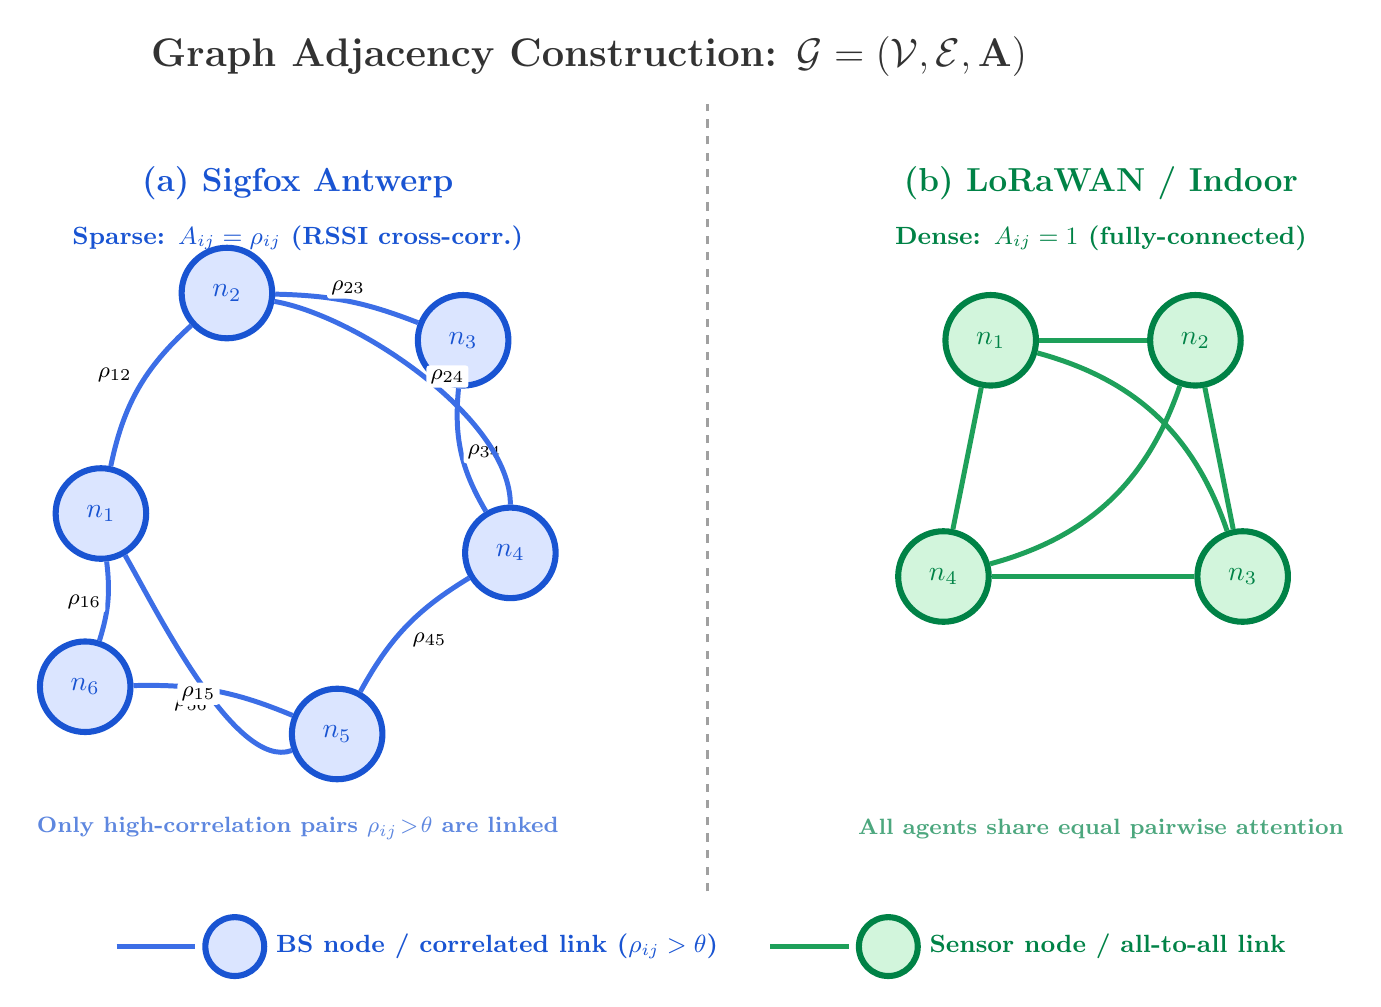
\begin{tikzpicture}[
  every node/.style={font=\bfseries},
  %% Node styles
  bsnode/.style={
    circle, draw=antcol, fill=antfill, line width=2.2pt,
    minimum size=1.15cm, font=\bfseries\normalsize, text=antcol,
    inner sep=0pt,
  },
  lrnode/.style={
    circle, draw=loracol, fill=lorafill, line width=2.2pt,
    minimum size=1.15cm, font=\bfseries\normalsize, text=loracol,
    inner sep=0pt,
  },
  %% Edge styles
  aedge/.style={draw=antedge, line width=1.8pt},
  ledge/.style={draw=loraedge, line width=1.8pt},
  %% Edge label style
  elabel/.style={
    font=\bfseries\footnotesize, fill=white,
    inner sep=1.5pt, rounded corners=1pt,
  },
]

%% =============================================================
%%  LEFT PANEL  —  Sigfox Antwerp: sparse RSSI-correlation graph
%% =============================================================
\node[bsnode] (a1) at (0.0,  0.0) {$n_1$};
\node[bsnode] (a2) at (1.6,  2.8) {$n_2$};
\node[bsnode] (a3) at (4.6,  2.2) {$n_3$};
\node[bsnode] (a4) at (5.2, -0.5) {$n_4$};
\node[bsnode] (a5) at (3.0, -2.8) {$n_5$};
\node[bsnode] (a6) at (-0.2,-2.2) {$n_6$};

%% Sparse edges — only high-correlation pairs connected
%% Use bend to produce gấp khúc / curved routing
\draw[aedge] (a1) to[bend left=18]
    node[elabel, midway, above left]  {$\rho_{12}$} (a2);

\draw[aedge] (a2) to[bend left=10]
    node[elabel, midway, above]       {$\rho_{23}$} (a3);

\draw[aedge] (a3) to[bend right=18]
    node[elabel, midway, right]       {$\rho_{34}$} (a4);

\draw[aedge] (a4) to[bend right=15]
    node[elabel, midway, below right] {$\rho_{45}$} (a5);

\draw[aedge] (a5) to[bend right=12]
    node[elabel, midway, below left]  {$\rho_{56}$} (a6);

\draw[aedge] (a6) to[bend right=12]
    node[elabel, midway, left]        {$\rho_{16}$} (a1);

%% Cross edge: n2 -- n4 (bent to avoid overlap)
\draw[aedge] (a2) to[out=-10, in=90, looseness=0.7]
    node[elabel, midway, right]       {$\rho_{24}$} (a4);

%% Cross edge: n1 -- n5 (bent, goes below center)
\draw[aedge] (a1) to[out=-60, in=200, looseness=0.6]
    node[elabel, midway, below]       {$\rho_{15}$} (a5);

%% Panel label
\node[font=\bfseries\large, text=antcol, align=center]
    at (2.5, 4.2) {(a) Sigfox Antwerp};
\node[font=\bfseries\small, text=antcol, align=center]
    at (2.5, 3.5)
    {Sparse: $A_{ij}=\rho_{ij}$ (RSSI cross-corr.)};
\node[font=\bfseries\footnotesize, text=antcol!70, align=center]
    at (2.5, -4.0)
    {Only high-correlation pairs $\rho_{ij}\!>\!\theta$ are linked};

%% =============================================================
%%  RIGHT PANEL  —  LoRaWAN / Indoor: fully-connected graph
%% =============================================================
\begin{scope}[xshift=10.5cm]

\node[lrnode] (b1) at (0.8,  2.2) {$n_1$};
\node[lrnode] (b2) at (3.4,  2.2) {$n_2$};
\node[lrnode] (b3) at (4.0, -0.8) {$n_3$};
\node[lrnode] (b4) at (0.2, -0.8) {$n_4$};

%% Outer cycle edges (straight)
\draw[ledge] (b1) -- (b2);
\draw[ledge] (b2) -- (b3);
\draw[ledge] (b3) -- (b4);
\draw[ledge] (b4) -- (b1);

%% Diagonal edges — bent (gấp khúc) to avoid overlap at center
\draw[ledge] (b1) to[bend left=28] (b3);
\draw[ledge] (b2) to[bend left=28] (b4);

%% Panel label
\node[font=\bfseries\large, text=loracol, align=center]
    at (2.2, 4.2) {(b) LoRaWAN / Indoor};
\node[font=\bfseries\small, text=loracol, align=center]
    at (2.2, 3.5)
    {Dense: $A_{ij}=1$ (fully-connected)};
\node[font=\bfseries\footnotesize, text=loracol!70, align=center]
    at (2.2, -4.0)
    {All agents share equal pairwise attention};

\end{scope}

%% =============================================================
%%  Vertical separator
%% =============================================================
\draw[sepgray, dashed, line width=1.2pt]
    (7.7, -4.8) -- (7.7, 5.2);

%% =============================================================
%%  Legend box  (bottom, spanning both panels)
%% =============================================================
\begin{scope}[yshift=-5.5cm]
  %% Left legend entry
  \draw[aedge]          (0.2, 0.0) -- (1.2, 0.0);
  \node[bsnode, scale=0.65] at (1.7, 0.0) {};
  \node[font=\bfseries\small, text=antcol, anchor=west] at (2.1, 0.0)
      {BS node / correlated link ($\rho_{ij}>\theta$)};

  %% Right legend entry
  \draw[ledge]          (8.5, 0.0) -- (9.5, 0.0);
  \node[lrnode, scale=0.65] at (10.0, 0.0) {};
  \node[font=\bfseries\small, text=loracol, anchor=west] at (10.4, 0.0)
      {Sensor node / all-to-all link};
\end{scope}

%% =============================================================
%%  Overall title (optional — can be removed if using figure caption)
%% =============================================================
\node[font=\bfseries\Large, text=titlegray, align=center]
    at (6.2, 5.8)
    {Graph Adjacency Construction: $\mathcal{G}=(\mathcal{V},\mathcal{E},\mathbf{A})$};

\end{tikzpicture}
\end{document}
